\documentclass[c,8pt,xcolor...,x11names]{beamer}
\usepackage{icclslides}
\usepackage[latin1]{inputenc}
\usepackage[british]{babel}
\usepackage{amssymb}
\usepackage{latexsym}
\usepackage{rotate}
\usepackage{tikz}
\usepackage{verbatim}
\usepackage{colortbl}
\usepackage{booktabs}
\usepackage{ulem}
% \usepackage{arydshln}
\usepackage{pdfpages}
\usepackage{graphicx} 
\usepackage{tikz}
\usetikzlibrary{positioning}

\tikzstyle{ele} = [circle, text centered, minimum width=1em, minimum height=3ex]

%% Uncomment to activate navigation symbols in the lower right of the pages:
\setbeamertemplate{navigation symbols}{}

\renewcommand{\Myauthor}{Emmanuelle Dietz}
\renewcommand{\Mytitle}{Howto: Introduction to Beamer}
\usepackage{showexpl} 

\lstloadlanguages{[LaTeX]Tex} 
\lstset{% 
	basicstyle=\ttfamily\small, 
	commentstyle=\itshape\ttfamily\small, 
	showspaces=false, 
	showstringspaces=false, 
	breaklines=true, 
	breakautoindent=true, 
	captionpos=t 
} 

\begin{document} 
	\begin{frame}
	\customtitle
	\begin{list2}
		\item What is {\sc Beamer}?
		\item How to produce a presentation?
		\item How to create overlays?
	\end{list2}
\end{frame}


\section{Introduction} % taken from Marek Seliger, Matthias Gerdts


\begin{frame}
\frametitle{Introduction}

{\color{blue}What is {\sc Beamer}?}
\begin{itemize}
	\item 
	{\sc Beamer} is a \LaTeX\ document class for producing slides
	\\
	created by Til Tantau at the Universit\"at zu L\"ubeck    
\end{itemize}
{\color{blue}Why using {\sc Beamer} to produce a presentation?}
\begin{enumerate}
	\item \LaTeX  based (all common \LaTeX\ commands can be used), \\
	thus reuse already written up material
	\item can also be used to create reports from
	presentations
	\item  easy overlays
	\item no external programs needed other than what you already use for \LaTeX
\end{enumerate}

\end{frame}


\begin{frame}
\vfill
\begin{LARGE}
\hfill Structure of a {\sc Beamer} Document \hfill 
\end{LARGE}
\vfill
\end{frame}

\subsection{Structure}

\begin{frame}
\frametitle{Structure}
\begin{minipage}[t]{0.48\linewidth}
\begin{enumerate}
\item The basic structure is the standard in \LaTeX. But:
\begin{itemize}
	\item<2-> Indicate that this document is of the {\sc Beamer}
	class.
	\item<3-> alternative themes: Frankfurt, Berlin, Bergen,Boadilla,
	Madrid, AnnArbor, Pittsburgh, Rochester,Antibes, ...
	% \item<4-> alternative color themes: seahorse, structure, albatross, beetle,
	% crane, dove, fly, seagull, wolverine, ...
	\item<4-> Main document
	\item<5-> Declare each slide (\textit{frame}) you want to create.
	\item<6-> Sections are used outside of the frame environment.
	
\end{itemize}
% 
\end{enumerate}
\end{minipage}\hfill
\begin{minipage}[t]{0.48\linewidth}
{\ttfamily
\alert<2>{\textbackslash documentclass\{beamer\}} \\
\alert<3>{\textbackslash usetheme\{Warsaw\}} \\
\% additional options here 
\\ [12pt]
\alert<4>{\textbackslash begin\{document\}}
\\ [12pt]
\alert<6>{\textbackslash section\{Section 1\}} \\
\alert<5>{\textbackslash begin\{frame\}}\\
\qquad \textbackslash frametitle\{title\}\\[12pt]
\% slide content in standard \LaTeX \\ [12pt]
\alert<5>{\textbackslash end\{frame\}} \\ [12pt]
\alert<6>{\textbackslash subsection\{Subsection 1\}} \\ [12pt]
\alert<4>{ \textbackslash end\{document\}}
}
\end{minipage}
\end{frame}

\subsection{Titlepage}

\begin{frame}[containsverbatim] \frametitle{Titlepage}

\begin{LTXexample}
\documentclass{beamer}
\usetheme{Montpellier}
\usepackage{array}
\usepackage{graphicx}

\title{Howto: Introduction to Beamer}
\author{Emmanuelle Dietz}
\institute{TU Dresden}
\date{May 14, 2012}

\begin{document}
\maketitle

\end{document}
\end{LTXexample} 
\end{frame}

\subsection{Sections}

\begin{frame}
\frametitle{Sections}

\begin{minipage}[t]{0.48\linewidth}
\tableofcontents
\end{minipage}\hfill
\begin{minipage}[t]{0.48\linewidth}
{\ttfamily
... \bigskip \\
\textbackslash section\{Introduction\} \\
... \bigskip \\
\textbackslash section\{Basics of Beamer\} \\
... \bigskip \\
\textbackslash subsection\{Basic Structure\} \\
\\
\textbackslash subsection\{Titlepage\} \\ }

\end{minipage}\hfill

\end{frame}


\section{Alerts}
\begin{frame}[fragile] \frametitle{Alerts}
We can emphasize portions of our slide using alerts. \\
\bigskip 
\begin{minipage}[t]{0.48\linewidth}
\begin{semiverbatim}
\\begin\{itemize\}
\\item \alert{\\alert\{important item\}}
\\item item 
\\item item
\\end\{itemize\}
\end{semiverbatim}
\end{minipage}
\hfill
\begin{minipage}[t]{0.48\linewidth}
\begin{itemize}
\item \alert{important item}
\item item 
\item item
\end{itemize}
\end{minipage}
\end{frame}

\section{Overlays}

\begin{frame}
\vfill
\begin{LARGE}
\hfill Overlays \hfill 
\end{LARGE}
\vfill
\end{frame}

\subsection{Pause}

\begin{frame}[fragile]
\frametitle{Pause}
\textbackslash pause creates stopping points so one frame can be
uncovered piecewise.
% It can be used, e.g. 
\\ \bigskip
\begin{minipage}[t]{0.48\linewidth}
\begin{verbatim}
\begin{itemize}
\item This item first \pause
\item This item second \pause
\item This item third
\end{itemize}
\end{verbatim}
\end{minipage}
\hfill
\begin{minipage}[t]{0.48\linewidth}\pause
\begin{itemize} 
\item This item first \pause
\item This item second \pause
\item This item third
\end{itemize}
\end{minipage}

\end{frame}

\subsection{Lists}

\begin{frame}[fragile]
\frametitle{Lists}
\begin{minipage}[t]{0.48\linewidth}
\begin{verbatim}
\begin{itemize}
\item<1-> This item first
\item<3-> This item third
\item<2-> This item second
\end{itemize}
\end{verbatim}
\end{minipage}
\hfill 
\begin{minipage}[t]{0.48\linewidth}
\begin{itemize}
\item<2-> This item first
\item<4-> This item third
\item<3-> This item second
\end{itemize} 
\end{minipage} \bigskip \\
\uncover<5->{
Note that the order is given by
\begin{semiverbatim}
\begin{itemize}
\item  Show  <1>  \textit{only} on slide 1
\item Show <1-> on slide 1 onwards
\item Show <1-4,6-8> on every slide except 5
\end{itemize}
\end{semiverbatim}
}
\end{frame}

% \subsection{Overlays with lists}

\begin{frame}[fragile]
\frametitle{Emphasize Text}
Parts of the slides can be emphasized using overlays with alerts or
color specifications. \\
\bigskip 
\begin{minipage}[t]{0.48\linewidth}
\begin{semiverbatim}
\\begin\{itemize\}
\\item \alert{\\alert\{important item\}}
\\item item 
\\item item
\\end\{itemize\}
\end{semiverbatim}
\end{minipage}
\hfill 
\begin{minipage}[t]{0.48\linewidth}
\uncover<2->{
\begin{itemize}
\item \alert{important item}
\item item 
\item item
\end{itemize}
\end{minipage}}
\vfill 
\begin{minipage}[t]{0.48\linewidth}
\begin{semiverbatim}
\uncover<3->{
\\begin\{itemize\}
\alert<5>{\\item \\alert<1>\{first important item\}}
\alert<7>{\\item \{\\color<3>\{blue\}\{third item\}\}}
\alert<6>{\\item \\alert<2>\{second important item\}}
\\end\{itemize\} }
\end{semiverbatim}
\end{minipage}
\hfill
\uncover<4->{
\begin{minipage}[t]{0.48\linewidth}
\bigskip
\begin{itemize}
\item \alert<5>{first important item}
\item {\color<7>{blue}{third item}}
\item \alert<6>{second important item}
\end{itemize}
\end{minipage}}

\end{frame}

\begin{frame}
\vfill
\begin{LARGE}
\hfill Overlays for Non-Lists \hfill 
\end{LARGE}
\vfill
\end{frame}

\begin{frame}[fragile]

\frametitle{Non-Lists}

For non-lists there are several alternatives:
\begin{itemize}
\item \textbackslash onslide
\item \textbackslash only
\item \textbackslash visible
\item \textbackslash uncover
\end{itemize}
\end{frame}

\subsubsection{\textbackslash only and \textbackslash
uncover}

\begin{frame}[fragile] \frametitle{Overlays for Non-Lists}

\textbackslash only
\begin{semiverbatim}
\alert<2>{\\only<1>\{Initial text.\}}
\alert<3>{\\only<2>\{Replaced by this on second slide.\}}
\alert<4>{\\only<3>\{Replaced again by this on third slide.\}}
\end{semiverbatim}
\bigskip 
\only<2>{Initial text.}
\only<3>{Replaced by this on second slide.}
\only<4>{Replaced again by this on third slide.}
\bigskip
\uncover<5->{
\textbackslash uncover}
\begin{semiverbatim}
\uncover<5->{
\alert<6>{\\uncover<1>\{Text shown on slide 1.\}}
\alert<7>{\\uncover<2>\{Text shown on slide 2.\}}
\alert<8>{\\uncover<3>\{Text shown on slide 3.\}}}
\end{semiverbatim}
\bigskip 
\uncover<6>{Text shown on slide 1.}
\uncover<7>{Text shown on slide 2.}
\uncover<8>{Text shown on slide 3.}

\end{frame}

\subsubsection{Example with Tikz}

\begin{frame}[fragile] \frametitle{Overlays with Tikz}
\begin{minipage}[t]{0.48\linewidth}\footnotesize
\begin{semiverbatim} 
\alert<2>{\\node (l1)  [circle, draw];}

\alert<4>{\\uncover<3->\{
\\node (t2) [left=6mm of l1] {};
\\node (l2) [circle,draw,below=3mm of t2];

\\node (t3) [right=12mm of l1] {};
\\node (l3) [circle,draw,below=3mm of t3];\}}

\alert<6>{\\uncover<5->\{
\\node (t4) [left=6mm of l2] {};
\\node (l4) [circle,draw,below=3mm of t4];

\\node (t5) [right=6mm of l2] {};
\\node (l5) [circle,draw,below=3mm of t5];

\\node (t6) [left=6mm of l3];
\\node (l6) [circle,draw,below=3mm of t6];
\\node (t7) [right=6mm of l3];
\\node (l7) [circle,draw,below=3mm of t7];\}}

\alert<3>{\\uncover<2->\{
\\draw (l1) -- (l2); \\draw (l1) --(l3);\}}

\alert<5>{\\uncover<4->\{
\\draw (l2) -- (l4); \\draw (l2) -- (l5);

\\draw (l3) -- (l6); \\draw (l3) -- (l7);\}}
\end{semiverbatim}
\end{minipage}
\hfill
\begin{minipage}[t]{0.48\linewidth}
\bigskip 
% \tikzstyle{ele} = [circle, text centered, minimum width=1em, minimum
%height=3ex]
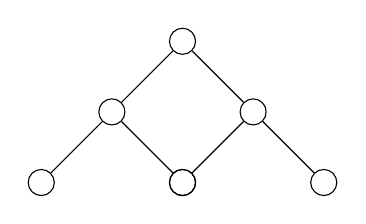
\begin{tikzpicture}
% tree
% root 
\uncover<2->{\node (l1)  [circle, draw] {};}

\uncover<4->{
\node (t2) [left=6mm of l1] {};
\node (l2) [circle,draw,below=6mm of t2] {};

\node (t3) [right=6mm of l1] {};
\node (l3) [circle,draw,below=6mm of t3] {};
}

\uncover<6->{
\node (t4) [left=6mm of l2] {};
\node (l4) [circle,draw,below=6mm of t4] {};

\node (t5) [right=6mm of l2] {};
\node (l5) [circle,draw,below=6mm of t5] {};

\node (t6) [left=6mm of l3] {};
\node (l6) [circle,draw,below=6mm of t6] {};
\node (t7) [right=6mm of l3] {};
\node (l7) [circle,draw,below=6mm of t7] {};}


% connections
\uncover<3->{
\draw (l1) -- (l2);
\draw (l1) --(l3);}

\uncover<5->{
\draw (l2) -- (l4);
\draw (l2) -- (l5);

\draw (l3) -- (l6);
\draw (l3) -- (l7);}

\end{tikzpicture} 
\end{minipage}
\end{frame}



\begin{frame}[fragile]
\frametitle{Overlays with Verbatim}

Semiverbatim allows using verbatim with overlays. This requires the
option [fragile]: \begin{verbatim}
\begin{frame}[fragile]
\end{verbatim}
\uncover<2->{
Example \bigskip \\
\begin{minipage}[t]{0.58\linewidth}
\begin{semiverbatim} \footnotesize
\\begin\{semiverbatim\} \newline
\textbackslash alert<3>\{\textbackslash
\textbackslash alert<2>\{important item\}\} \newline
\\end\{semiverbatim\}
\end{semiverbatim}
\end{minipage}
\hfill  
\begin{minipage}[t]{0.4\linewidth} 
\vspace{1pt}
\begin{semiverbatim} \footnotesize 
\alert<3>{\\alert<2>\{important item\}}
\end{semiverbatim}
\end{minipage}
}


\end{frame}

\begin{frame}[fragile]
\frametitle{Other Stuff}
\begin{itemize}

\item Suppress naviation symbols \\
\begin{verbatim}
\setbeamertemplate{navigation symbols}{}
\end{verbatim} 
\item Suppress the headlines, footlines, and sidebars \\
\begin{verbatim}
\begin{frame}[plain]
\end{verbatim}
\item Add ``handout'' parameter for slides without overlays (e.g. for printout) \\
\begin{semiverbatim}
\\documentclass[..., handout]\{beamer\}
\end{semiverbatim}

%\item semiverbatim to show latex code in the presentation (option
\item Include blank black slide \\
\begin{semiverbatim}
\\bgroup
\\setbeamercolor\{background canvas\}\{bg=black\}
\\begin\{frame\}[plain]\{\}
\\end\{frame\}
\\egroup
\end{semiverbatim}
\end{itemize}
\end{frame}


\section{Further Information}

\begin{frame}
\frametitle{Further Information}
\begin{itemize}
\item Till Tantau, Joseph Wright, Vedran Mileti\'{c}: The {\sc beamer}
class \\ \url{
http://www.ctan.org/tex-archive/macros/latex/contrib/beamer/doc/beameruserguide.
pdf}
\item Charles T. Batts: A Beamer Tutorial in Beamer \\
\url{http://www.scribd.com/doc/47716986/Charles-Batts-Beamer-Tutorial} 
\end{itemize}

\end{frame}

\section{References}

\begin{frame}
\frametitle{References}

\begin{itemize}
\item Charles T. Batts: A Beamer Tutorial in Beamer \\
\url{http://www.scribd.com/doc/47716986/Charles-Batts-Beamer-Tutorial}
\item Matthias Gerdts: Introduction to Beamer \\ \url{
http://www.unibw.de/lrt1/gerdts/lehre/zusatzmaterial-und-links/beamer-intro.pdf}
\item Gonzalo Rivero: Presentations in \LaTeX\ , Introduction to the  {\sc
beamer} class \\
\url{www.nyu.edu/projects/politicsdatalab/latex/beamer\_nyu.pdf}
\item Till Tantau, Vedran Mileti\'c, Joseph Wright: Creating Overlays\\
\url{
http://get-software.net/macros/latex/contrib/beamer/doc/beamerug-overlays.tex}
\end{itemize}

\end{frame}

\bgroup
\setbeamercolor{background canvas}{bg=black}
\begin{frame}[plain]{}
\end{frame}
\egroup

\end{document}
